\documentclass{article}
\usepackage[utf8]{inputenc}
\usepackage[english]{babel}
\usepackage[legalpaper, portrait, margin=1in]{geometry}
\usepackage{setspace}
\onehalfspacing
\usepackage{parskip}
\setlength{\parindent}{0cm}
\usepackage{enumitem}
\setlist{nosep}
\usepackage{hyperref}
\usepackage{graphicx}

\hypersetup{
  	colorlinks,
	citecolor=black,
	filecolor=black,
	linkcolor=black,
	urlcolor=black
}
\title{%
  Polis DAO Manifesto \\
  \large Functional DAO for Open Source cryptocurrency projects.}
\author{
  Berrueta, Enrique\\
  \texttt{eabz@polispay.org}
  \and
  Bustos, Ricardo\\
  \texttt{eros@polispay.org}
}
\date{June 2020}

\begin{document}

\maketitle

	\begin{abstract}
    A DAO is a ``Decentralized Autonomous Organization`` or a corporation without a central authority that can be governed by a multi-party of authorized members chosen by a bigger community. Throughout the years, several DAO and governance attempts have been made since cryptocurrencies started. From Dash to Ethereum's ``The DAO``, all these organizations have had various problems, from lack of organization to falling into outright centralization. After pondering it, I've come to propose a new solution for creating a functional DAO, that will not only be decentralized but also organized and inclusive.
	\end{abstract}

\newpage

\tableofcontents


\newpage

\section{Structure}

The DAO will be based upon five fundamental pillars, of which there will be a person in charge chosen by the community for each pillar:

\begin{itemize}
  \item Technology.
  \item Community.
  \item Business.
  \item Adoption.
  \item Marketing.
\end{itemize}

\begin{figure}[h]
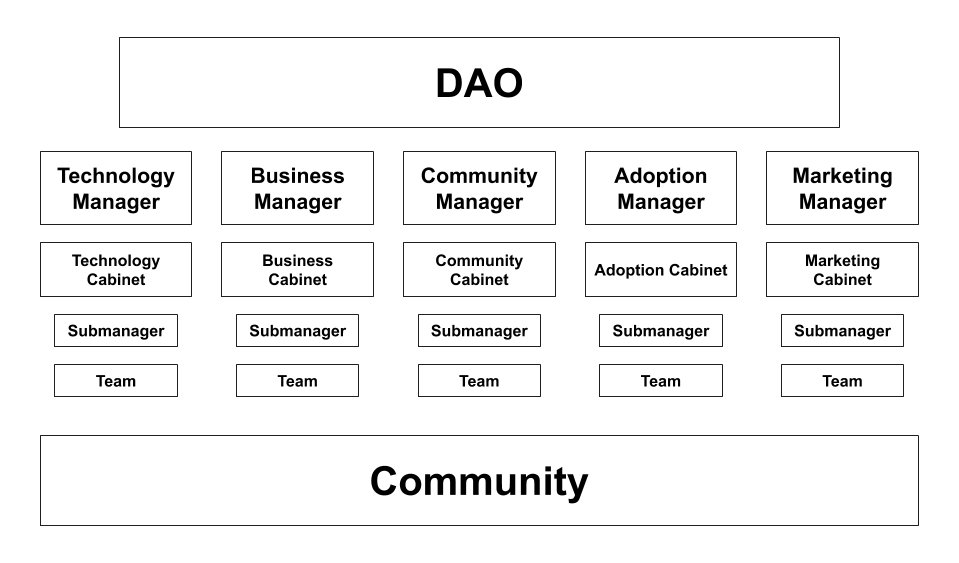
\includegraphics[scale=0.4]{img/dao_structure_en.png}
\centering
\caption{Basic organization model of the DAO}
\end{figure}

Each person in charge, who from now will be called ``Manager``, will be eligible based on their prestige on the community. They will present a proposal to the community, detailing their proposals for the cycle of command, which will last a year.

On their proposal, each manager must delineate the following points:

\begin{itemize}
  \item Improvement proposals.
  \item Members of their team (cabinet).
  \item Strategies they will employ to achieve their proposals.
  \item Why should the community vote for them.
  \item Detailed roadmap with specific timetables established.
\end{itemize}

Managers will be eligible for reelection for as many times as they desire to, as long as the community agrees with them.

\section{Keys}

Since the entire DAO is referred to as a cryptocurrency ecosystem, everything related to voting and decision making should be done using a DAO Key. These Keys are secured by the manager and access is granted/removed during the DAO Voting cycles or the execution of a safety mechanism.

These Keys are changed over the DAO cycles if a manager position changes on a voting cycle or a security mechanism. This Key will be the receiver of the coins for the specific area and will be used to unlock the coins (together with the other 5 managers) on the community proposals and the over budget.

\section{Treasury}

For a DAO to properly work as an organization it is completely required to have funds. Since it is not possible to support it based on donations, here we propose a funding model that guarantees equitable funding and a distribution model for each area.

The 20\% of the monthly coins emitted will be locked into an account used for the DAO.

These funds will be distributed in three categories:

\begin{itemize}
  \item 10\% to the DAO areas.
  \item 5\% for community proposals.
  \item 5\% locked for areas over-budget.
\end{itemize}

The DAO Areas budget will be distributed based on the following proportions:

\begin{itemize}
  \item 30\% Technology.
  \item 10\% Community.
  \item 20\% Business.
  \item 20\% Marketing.
  \item 20\% Adoption.
\end{itemize}

The 5\% for community proposals should be distributed based on the manager decision. They will decide when a proposal should be funded.

The 5\% for areas over-budget should be used based on the manager decision to increase a specific area budget for a specific period.

The funds will be deposited each month to the current manager Key by the network automatically.

The community  over budget funds will be deposited to a multi-signature generated key to make sure only 3 out of 5 managers are able to withdraw those funds.

Community proposals must detail:

\begin{itemize}
  \item Amount of budget required.
  \item Action plan.
  \item Detailed budget of costs.
\end{itemize}

\section{Cycles}

The DAO is functionality is determined by time cycles. There are only three cycles that involve decisions on different moments.

\subsection{Voting Cycle}

The voting cycle starts each year the 20 of January. This process takes around 2 or 3 weeks and the idea is to have a election campaign on which old managers and new members that want to get involved technically to the DAO must do their proposals and road-maps to be qualified.

This cycle has four phases:

\begin{itemize}
  \item Candidates Postulations.
  \item Candidates Proposals.
  \item Elections Preparations.
  \item Voting.
\end{itemize}

\subsection{Budgeting Cycle}

Once the managers are chosen they must provide a proper budget on which they will operate the next three months. This budget should be presented by the Business Manager each three months including the budget and the real expenses to provide the community with transparent information.

\subsection{Reporting Cycle}

Alongside the Budget cycles, each manager should create a report on its own areas about the achievements of the 3 months work to the managers and to the Community.

If a manager doesn't upload the report to the network, their key us automatically removed from the DAO Keys.

\section{Areas}

\subsection{Technology}

The manager in charge of technology will be responsible for recruiting and training developers to follow the DAO's technical road-map.

The manager will have the following duties:

\begin{itemize}
  \item Cryptocurrency technology development.
  \item Use-cases development.
  \item Third-party libraries.
  \item Documentation and maintenance.
\end{itemize}

Alongside the Community Manager is in charge of the proper functionality and documentation of the following services:

\begin{itemize}
  \item Official block explorers.
  \item Websites.
  \item Guides.
  \item Forums.
  \item Internal resources.
\end{itemize}

\subsection{Community}

The manager in charge of the community will be responsible for the community and the integrity and correctness of the information displayed on the multiple channels.

The manager will have the following duties:

\begin{itemize}
  \item Communication and social media.
  \item Documentation and maintenance.
  \item User's technical support and security best practices.
  \item Correct branding and design.
\end{itemize}

Alongside the technology manager is in charge of the proper functionality and documentation of the following services:

\begin{itemize}
  \item Official block explorers.
  \item Websites.
  \item Guides.
  \item Forums.
  \item Internal resources.
\end{itemize}

\subsection{Business}

The manager in charge of business is responsible for establishing new partnerships with other projects and following the community proposals.

The manager will have the following duties:

\begin{itemize}
  \item Partnerships.
  \item Administration and budget transparency.
  \item Community proposals follow up.
\end{itemize}

\subsection{Adoption}

The manager in charge of adoption will be responsible for bringing merchants into the project as well as getting new developers to use the technology for their purposes and organize events to attract the usage of the network.

The manager will have the following duties:

\begin{itemize}
  \item Merchants adoption.
  \item Developers adoption.
  \item Public Relationships and Information Office.
\end{itemize}

\subsection{Marketing}

The manager in charge of marketing will be responsible for looking for outreach spaces as long as to bring the other managers with analytic and marketing strategies.

The manager will have the following duties:

\begin{itemize}
  \item Marketing strategies lines and road-maps.
  \item Analytic and intelligence reports.
  \item Advertising spaces.
\end{itemize}

\section{Safe Mechanisms}

Since the DAO implies trusting the organization to known members, safe-mechanisms should be developed based on the discussion and security of the network.

We only envisioned two possible cases on which an issue to the DAO structure or funds can happen. To cover those cases we built the following safe mechanism.

\subsection{Manager Banning}

If under any circumstance the managers want to remove a member, they can use their DAO Key to create a signed message to the network for the removal of the key from the DAO Keys. For this mechanism to execute it requires at least 3 of 5 possible signatures.

\subsection{DAO Banning}

This mechanism is executed by the community, it implies that some way the managers are not doing their work correctly or the entire DAO is taken by a group that is harming the entire ecosystem.

Community members can create a signed message with a proof-of-possession of a number of coins, once the threshold passes the 30\% of the total coin supply, all the DAO keys are removed and a emergency voting cycle starts.

\end{document}
